\documentclass[conference]{IEEEtran}
\usepackage{cite}
\usepackage{amsmath,amssymb,amsfonts}
\usepackage{algorithmic}
\usepackage{graphicx}
\usepackage{textcomp}
\usepackage{xcolor}
\usepackage{float}
\usepackage{listings} % <翟> 加了一个库用来展示代码
\def\BibTeX{{\rm B\kern-.05em{\sc i\kern-.025em b}\kern-.08em
    T\kern-.1667em\lower.7ex\hbox{E}\kern-.125emX}}
\begin{document}

\title{COMP3023J Software Methodology Research Group11\\}

\author{\IEEEauthorblockN{1\textsuperscript{st} Jinpeng Zhai}
\IEEEauthorblockA{\textit{Software Engineering Year of 2021} \\
\textit{Beijing-Dublin International College}\\
Beijing, China \\
jinpeng.di@ucdconnect.ie}
\and
\IEEEauthorblockN{2\textsuperscript{nd} Ziqi Yang}
\IEEEauthorblockA{\textit{Software Engineering Year of 2021} \\
\textit{Beijing-Dublin International College}\\
Beijing, China \\
ziqi.yang@ucdconnect.ie}
\and
\IEEEauthorblockN{3\textsuperscript{rd} Yiran Zhao}
\IEEEauthorblockA{\textit{Software Engineering Year of 2021} \\
\textit{Beijing-Dublin International College}\\
Beijing, China \\
ZhaoYiran@emails.bjut.edu.cn}
}

\maketitle

\begin{abstract}
This paper, authored by Group 11, serves as a midterm checkpoint for the COMP3023J Software Methodology course research assignment. It is important to note that a comprehensive abstract will be provided upon the completion of the entire manuscript.
\end{abstract}

\begin{IEEEkeywords}
Python, tracing, visualization
\end{IEEEkeywords}

\section{Introduction}
% python的流行性和广泛应用
Python is widely recognized as one of the most popular programming languages in contemporary computing. Its popularity stems from its exceptional flexibility, ease of learning, and the extensive selection of libraries available\cite{saabith2019python}. Python's widespread adoption is not limited to well-established fields such as web development, data analytics, and scientific computing; it has also gained prominence in emerging areas, notably in the domain of machine learning\cite{zhang2020python}. This increasing popularity has led to a growing community of developers and researchers.

% python项目中的挑战,过渡到对大型python项目进行分析和优化的重要性。这部分其实如果写具体可以写成两段
However, as Python projects expand in size and complexity, they encounter fresh challenges associated with both development and maintenance. These challenges encompass intricacies in code organization, the emergence of ``hot code" leading to performance bottlenecks, and the escalating intricacies of ongoing maintenance\cite{peng2021empirical}. Consequently, there arises a compelling need for code analysis and optimization for large Python projects\cite{ray2014large}.

% 先前的研究背景?写了一下关于trace代码追踪和分析的。然后还有可视化的。这也可以详细写分成两段。
Previous studies have emphasised the efficacy of employing code tracing and code coverage techniques within Python projects in tackling these problems. Code tracing refers to the action of following the flow of program execution. It shares some similarities with deterministic profiling and debugging, in that in the context of Python, this is usually accomplished via placing a hook function into the Python interpreter via the provided sys.settrace() method, that is then called to record the exact detail of program execution. Among these, CPython's Lib.trace.py module provides robust capabilities in tracing the execution of native Python code\cite{aakerblom2014tracing}. This module adeptly traces function calls and furnishes comprehensive code coverage reports, thus facilitating the identification of inadequately tested code and performance bottlenecks. \par
 
% 这段大概扩充一下,因为我们组相对来讲是偏向于visualization的
Simultaneously, a growing trend in recent years has witnessed the adoption of visualization tools to enhance code analysis, presenting findings in an intuitively accessible format\cite{cao2021research,fernandez2023empirical}. This trend serves to further enhance code quality and bolster the maintainability of large Python projects.\par

Of note is that due to the converging interest in developing better techniques for the visualizatio of profiling results, in recent years popular visualization packages have instead opted for extending either the \textit{pdb}, the Python debugger module, or various deterministic profilers, traditionally either the \textit{profile} or the \textit{cProfile} packages. The merits of some of these options will be explored later in this report.\par


% 最后是我们的研究目的,这个后期分析的目标定了之后要重写一下
Consequently, this research aims to explore and compare various options for tracing Python code visualization, and demonstrate the use of these techniques for a better understanding of complex Python projects.\par

\section{Previous Art} % <翟> Literature Review -> Previous Art
% <翟> 这个是前几天一直在忙的那个python自带的trace,讲一下它的大概情况
Lib/trace.py is the tool bundled with CPython, the reference implementation for Python language\cite{cpythonlibtracepy}. Written in the early 2000s, it has been part of the official library from as early as Python 2.2. It provides both program execution tracing and code coverage analysis functionality, and even a limited profiling ability. Implementation-wise, it attaches a tracing funciton, written in Python, that is attached to the evaluation mechanism in the underlying Python interpreter, and is called during the normal execution of CPython\cite{trace}. As for usability, it supports both programmatic invocation and via the command line.\par

Coverage.py is a more recent third-party code coverage package that started in 2009 and has apparently gained some official endorsement\cite{batchelder_2023_coveragepy}. It employs a similar strategy, but differs in its implementation, specifically using a trace function in C. This avoids the overhead involved with converting C data types to Python ones and calling a Python function from C code for each evaluation, in exchange for some overhead at the end of tracing \cite{a2011_how}.
Through this, the impact of tracing on program execution can almost be eliminated. Given the package's focus on coverage analysis, it provides less exportable information with regard to program execution flow besides coverage information. From a users perspective, although execution is limited to command line invocation, it supports more modern formats for reporting, including in HTML and such. \par

Various Python profilers, in particular profiling tools bundled with CPython as part of the standard library, the \textit{profile} and the C implementation \textit{cProfile} are also of some interest. As deterministic profilers, they records and expose the Python call stack for each evaluation, allowing program execution tracing to be inferred. Due to the wealth of information recorded, over the years, many projects that visualizes program execution has built upon its output. Notable ones includes: \par
\begin{enumerate}
    \item RunSnakeRun. Generates a variation of tree map using performance statistics. Call relation implied by geometrical relations.
    \item GProf2Dot and PyCallgraph. Generates a directed arrow-and-box graph with performance statistics, broken down based on call relations.
\end{enumerate}
Of note is that not all profilers are suitable for our purposes. In particular, non-deterministic profilers works by sampling, at set intervals, the memory layout of the Python interpreter, thus they are suitable for low overhead programm profiling, but unsuitable when capturing function calls for analysis are required, since there is no guarantee of the completeness of the resulting capture. Solutions based on these will be ignored for the purpose of this study.

\section{Methodology}
Describe the way that you do your own research and how you are going to explore the thesis statement that you made. 

\section{Experiments and results}


Analyze experimental results. 
\section{Discussion}
Explore the results and talk about the implications that the results have upon the entire body of research which existed. 

\section{Conclusion}
General statement and ending thoughts about the topic. 


\section{Project Management}
% 文档里面的要求:
% Describe organizational matters that you used for effective teamwork (e.g., organizing group meetings, managing shared resources and resolving ambiguities). 
% List the projected milestones and dates using Gantt charts. 
% Provide an itemized list of each team member's contribution. Quantify each team member's contribution as a percentage. 
% Discuss the possible directions for future work on your research. 

Throughout the course of this research project, effective project management practices were diligently implemented to ensure the successful execution of the study and the attainment of its research objectives. This section offers insights into key aspects of project management, including team management, the presentation of milestones through Gantt charts, individual team member contributions, and potential future research directions.

\subsection{Team Management}
Effective team management is paramount for the success of a research project, ensuring that all team members work cohesively towards common goals. In the context of this study, several strategies were meticulously employed to promote efficient teamwork:

\begin{itemize}
    \item \textbf{Cohesive and Collaborative Team:} Our research team thrived on a culture of cohesiveness and collaboration. Team members actively engaged in learning about each other's work, encouraging knowledge sharing, and fostering an environment of continuous improvement. Mutual respect, inclusivity, and honesty were the cornerstones of our interactions. We recognized and celebrated each team member's distinct attributes and strengths, resulting in a balanced and complementary team.
    \item \textbf{Regular Team Meetings:} The project team scheduled and adhered to regular meetings to facilitate thorough discussions on various aspects of the research. These meetings became a platform for deliberating project progress, addressing issues, and setting forth objectives for the upcoming stages. The consistency of these meetings ensured that all team members were continuously aligned with the research objectives and were aware of the project's evolving dynamics.
    \item \textbf{Effective Team Organization:} Organizational structures significantly impact the decision-making process within a team. Effective communication is the cornerstone of our team management strategy. In addition to scheduled meetings, we established digital communication platforms, specifically WeChat and Telegram group chats, to facilitate real-time communication and information sharing among team members. These platforms allowed for swift discussions and collaborative decision-making, ensuring that everyone was on the same page regarding project developments. 
    \item \textbf{Shared Resource Management:} To facilitate efficient collaboration and resource accessibility, the research team adopted modern tools and platforms. A dedicated GitHub repository was established for streamlined code sharing and collaboration on experimental components. This central repository allowed team members to work on project software with version control and simplified issue tracking. Additionally, Overleaf, an online platform for collaborative writing, was used to create and edit the research paper collectively. This real-time collaboration improved the efficiency of document creation and review. These modern tools ensured easy access to project resources, including code and research documentation, enhancing collaboration, version control, and issue resolution for the success of the research project.
\end{itemize}

Our team management practices were instrumental in fostering a collaborative and productive environment, which ultimately played a pivotal role in the successful execution of this research project.  The harmonious teamwork, communication, and resource management strategies allowed us to efficiently navigate the complexities of the research process and achieve our project objectives.

\subsection{Milestone Showcase with the Gantt Chart}

\begin{figure*}[htbp]
\centerline{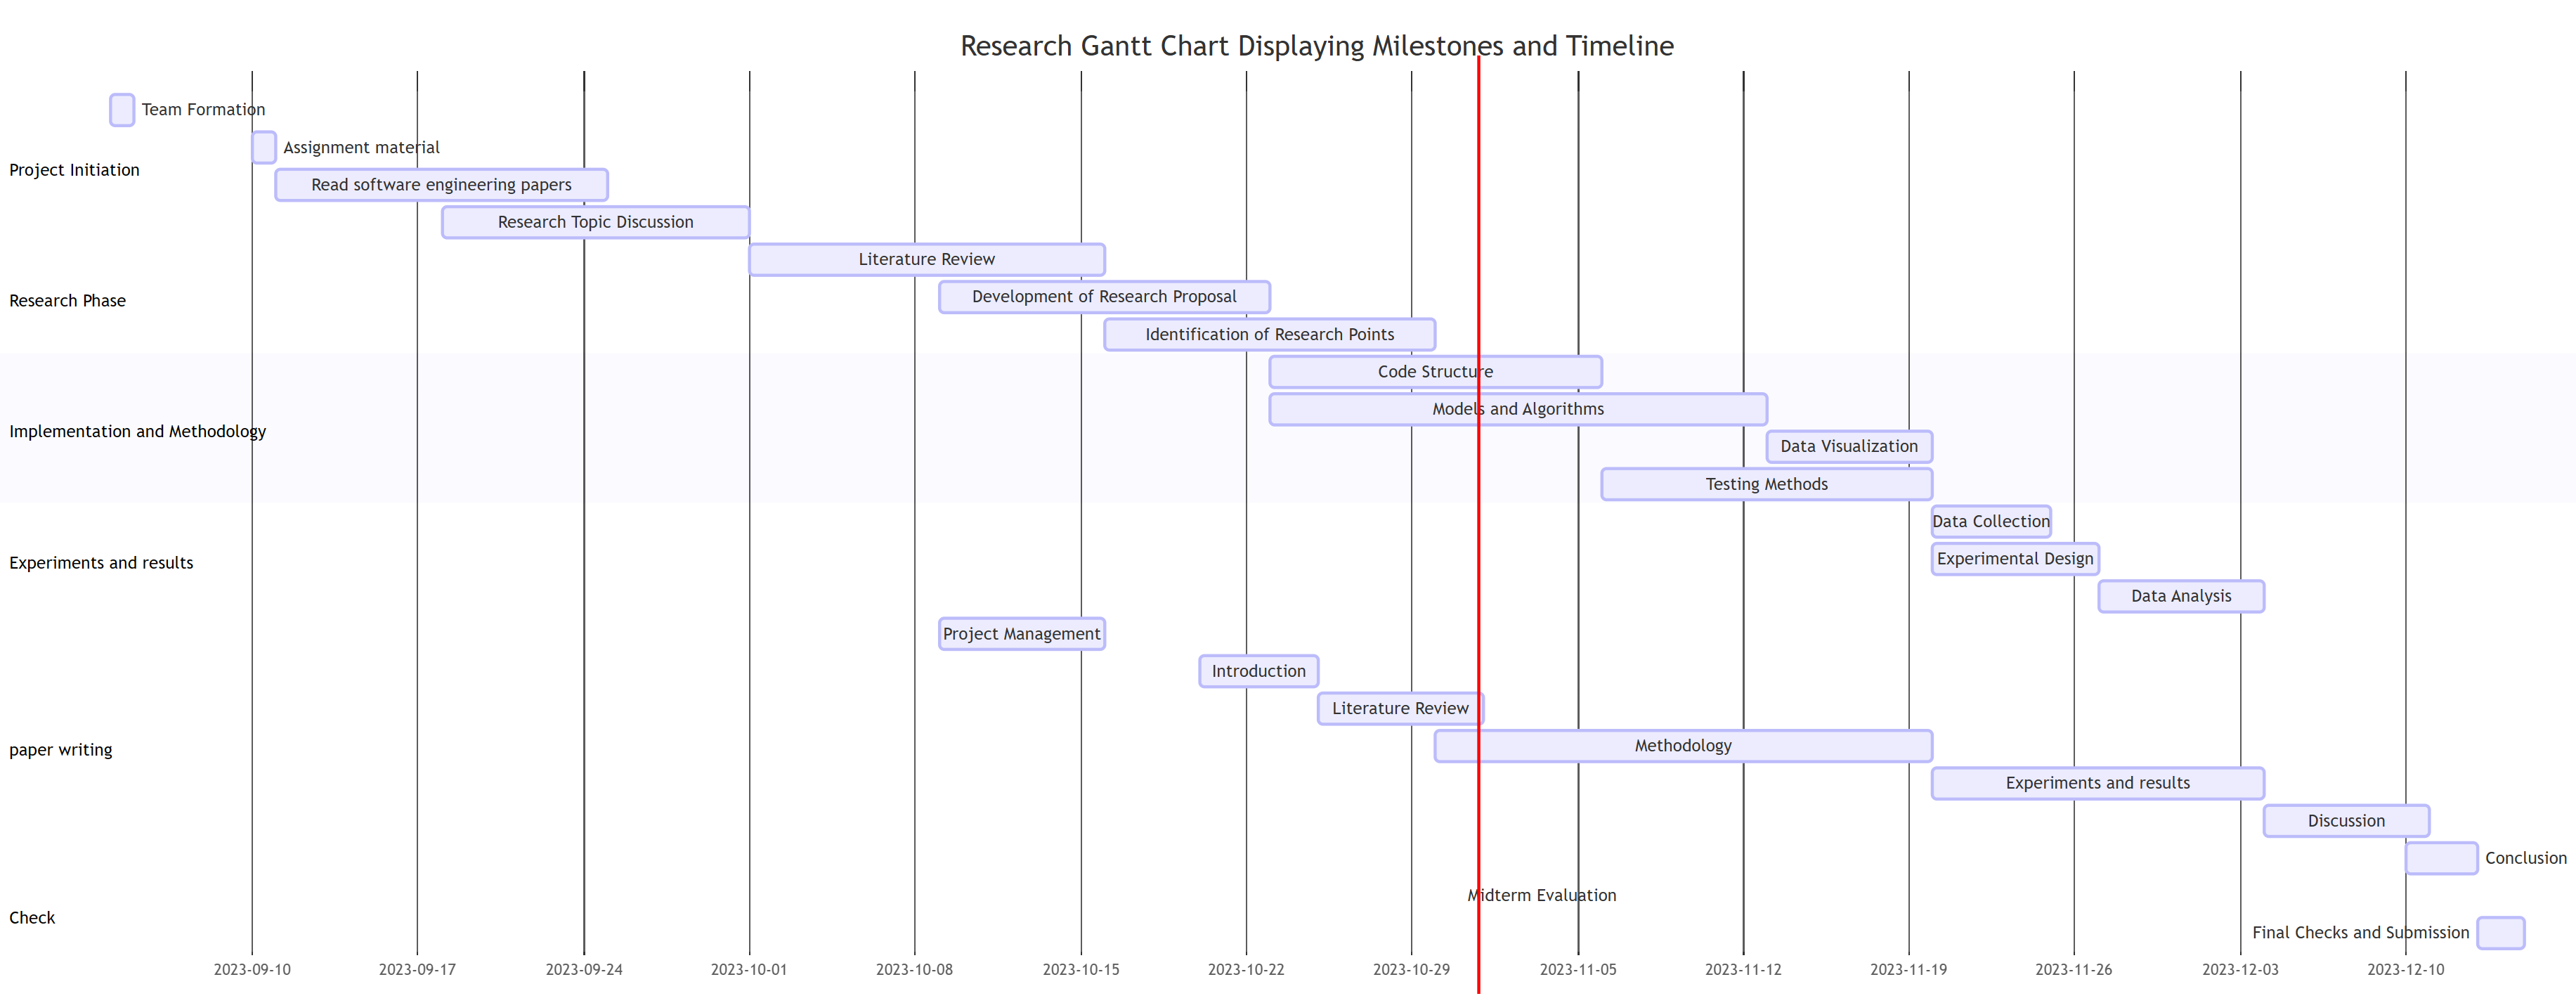
\includegraphics[scale=0.26]{figures/Gantt.png}}
\caption{Research Gantt Chart Displaying Milestones and Timeline}
\label{fig: Gantt}
\end{figure*}

As illustrated in Figure~\ref{fig: Gantt}, the Gantt chart is an instrumental graphical representation that offers a structured overview of the project's chronological progression and key milestones.  This visual representation is an essential tool for effective project management, aiding in the tracking of tasks, allocation of resources, and adherence to project timelines.

\subsection{Team Member Contributions}
Each member of the research team made substantial and equitable contributions to the success of the project. It is worth noting that the team unanimously acknowledges that each member's contributions to the research project were fundamentally equal and characterized by active engagement. Below is a detailed breakdown of the tasks and responsibilities that each team member undertook:

\begin{itemize}
    \item Jinpeng Zhai
    \begin{itemize}
        \item Actively engaged in the implementation of the research plan, transforming initial concepts into concrete project components.
        \item Took the lead in formulating and developing the research methodology, playing a crucial role in crafting the research approach presented in the paper.
        \item Contributed significantly to the writing of the research's methodology and approach sections in the paper, ensuring its thoroughness and accuracy.
    \end{itemize}
    \item Ziqi Yang
    \begin{itemize}
        \item Demonstrated proactiveness in conducting extensive research to identify available tools and the latest research methods.
        \item Presented innovative ideas for implementation and actively participated in the design and development phases of the research.
        \item Contributed to the creation of project components and the development of research solutions, enriching the research's technical foundation.
    \end{itemize}
    \item Yiran Zhao
    \begin{itemize}
        \item Formed and efficiently managed the research team, facilitating regular team meetings and fostering effective communication.
        \item Contributed to the research paper, including creating the overleaf template and drafting the introduction section and project management section.
        \item Thoroughly reviewed relevant literature, bringing a wealth of knowledge and insights to the research. Introduced innovative ideas and approaches that enriched the research process and contributed to the research's overall success.
    \end{itemize}
\end{itemize}

The entire team is in unanimous agreement that each member's commitment and contributions to the research project were equitable and integral to its success. The collaborative and complementary efforts of all team members were essential in achieving the project's goals.

\subsection{Future Research Directions}



% 下面是模板里面本来有的内容
% \section{TEMPLATE}
% \subsection{Maintaining the Integrity of the Specifications}

% The IEEEtran class file is used to format your paper and style the text. All margins, 
% column widths, line spaces, and text fonts are prescribed; please do not 
% alter them. You may note peculiarities. For example, the head margin
% measures proportionately more than is customary. This measurement 
% and others are deliberate, using specifications that anticipate your paper 
% as one part of the entire proceedings, and not as an independent document. 
% Please do not revise any of the current designations.

% \section{Prepare Your Paper Before Styling}
% Before you begin to format your paper, first write and save the content as a 
% separate text file. Complete all content and organizational editing before 
% formatting. Please note sections \ref{AA}--\ref{SCM} below for more information on 
% proofreading, spelling and grammar.

% Keep your text and graphic files separate until after the text has been 
% formatted and styled. Do not number text heads---{\LaTeX} will do that 
% for you.

% \subsection{Abbreviations and Acronyms}\label{AA}
% Define abbreviations and acronyms the first time they are used in the text, 
% even after they have been defined in the abstract. Abbreviations such as 
% IEEE, SI, MKS, CGS, ac, dc, and rms do not have to be defined. Do not use 
% abbreviations in the title or heads unless they are unavoidable.

% \subsection{Units}
% \begin{itemize}
% \item Use either SI (MKS) or CGS as primary units. (SI units are encouraged.) English units may be used as secondary units (in parentheses). An exception would be the use of English units as identifiers in trade, such as ``3.5-inch disk drive''.
% \item Avoid combining SI and CGS units, such as current in amperes and magnetic field in oersteds. This often leads to confusion because equations do not balance dimensionally. If you must use mixed units, clearly state the units for each quantity that you use in an equation.
% \item Do not mix complete spellings and abbreviations of units: ``Wb/m\textsuperscript{2}'' or ``webers per square meter'', not ``webers/m\textsuperscript{2}''. Spell out units when they appear in text: ``. . . a few henries'', not ``. . . a few H''.
% \item Use a zero before decimal points: ``0.25'', not ``.25''. Use ``cm\textsuperscript{3}'', not ``cc''.)
% \end{itemize}

% \subsection{Equations}
% Number equations consecutively. To make your 
% equations more compact, you may use the solidus (~/~), the exp function, or 
% appropriate exponents. Italicize Roman symbols for quantities and variables, 
% but not Greek symbols. Use a long dash rather than a hyphen for a minus 
% sign. Punctuate equations with commas or periods when they are part of a 
% sentence, as in:
% \begin{equation}
% a+b=\gamma\label{eq}
% \end{equation}

% Be sure that the 
% symbols in your equation have been defined before or immediately following 
% the equation. Use ``\eqref{eq}'', not ``Eq.~\eqref{eq}'' or ``equation \eqref{eq}'', except at 
% the beginning of a sentence: ``Equation \eqref{eq} is . . .''

% \subsection{\LaTeX-Specific Advice}

% Please use ``soft'' (e.g., \verb|\eqref{Eq}|) cross references instead
% of ``hard'' references (e.g., \verb|(1)|). That will make it possible
% to combine sections, add equations, or change the order of figures or
% citations without having to go through the file line by line.

% Please don't use the \verb|{eqnarray}| equation environment. Use
% \verb|{align}| or \verb|{IEEEeqnarray}| instead. The \verb|{eqnarray}|
% environment leaves unsightly spaces around relation symbols.

% Please note that the \verb|{subequations}| environment in {\LaTeX}
% will increment the main equation counter even when there are no
% equation numbers displayed. If you forget that, you might write an
% article in which the equation numbers skip from (17) to (20), causing
% the copy editors to wonder if you've discovered a new method of
% counting.

% {\BibTeX} does not work by magic. It doesn't get the bibliographic
% data from thin air but from .bib files. If you use {\BibTeX} to produce a
% bibliography you must send the .bib files. 

% {\LaTeX} can't read your mind. If you assign the same label to a
% subsubsection and a table, you might find that Table I has been cross
% referenced as Table IV-B3. 

% {\LaTeX} does not have precognitive abilities. If you put a
% \verb|\label| command before the command that updates the counter it's
% supposed to be using, the label will pick up the last counter to be
% cross referenced instead. In particular, a \verb|\label| command
% should not go before the caption of a figure or a table.

% Do not use \verb|\nonumber| inside the \verb|{array}| environment. It
% will not stop equation numbers inside \verb|{array}| (there won't be
% any anyway) and it might stop a wanted equation number in the
% surrounding equation.

% \subsection{Some Common Mistakes}\label{SCM}
% \begin{itemize}
% \item The word ``data'' is plural, not singular.
% \item The subscript for the permeability of vacuum $\mu_{0}$, and other common scientific constants, is zero with subscript formatting, not a lowercase letter ``o''.
% \item In American English, commas, semicolons, periods, question and exclamation marks are located within quotation marks only when a complete thought or name is cited, such as a title or full quotation. When quotation marks are used, instead of a bold or italic typeface, to highlight a word or phrase, punctuation should appear outside of the quotation marks. A parenthetical phrase or statement at the end of a sentence is punctuated outside of the closing parenthesis (like this). (A parenthetical sentence is punctuated within the parentheses.)
% \item A graph within a graph is an ``inset'', not an ``insert''. The word alternatively is preferred to the word ``alternately'' (unless you really mean something that alternates).
% \item Do not use the word ``essentially'' to mean ``approximately'' or ``effectively''.
% \item In your paper title, if the words ``that uses'' can accurately replace the word ``using'', capitalize the ``u''; if not, keep using lower-cased.
% \item Be aware of the different meanings of the homophones ``affect'' and ``effect'', ``complement'' and ``compliment'', ``discreet'' and ``discrete'', ``principal'' and ``principle''.
% \item Do not confuse ``imply'' and ``infer''.
% \item The prefix ``non'' is not a word; it should be joined to the word it modifies, usually without a hyphen.
% \item There is no period after the ``et'' in the Latin abbreviation ``et al.''.
% \item The abbreviation ``i.e.'' means ``that is'', and the abbreviation ``e.g.'' means ``for example''.
% \end{itemize}
% An excellent style manual for science writers is \cite{b7}.

% \subsection{Authors and Affiliations}
% \textbf{The class file is designed for, but not limited to, six authors.} A 
% minimum of one author is required for all conference articles. Author names 
% should be listed starting from left to right and then moving down to the 
% next line. This is the author sequence that will be used in future citations 
% and by indexing services. Names should not be listed in columns nor group by 
% affiliation. Please keep your affiliations as succinct as possible (for 
% example, do not differentiate among departments of the same organization).

% \subsection{Identify the Headings}
% Headings, or heads, are organizational devices that guide the reader through 
% your paper. There are two types: component heads and text heads.

% Component heads identify the different components of your paper and are not 
% topically subordinate to each other. Examples include Acknowledgments and 
% References and, for these, the correct style to use is ``Heading 5''. Use 
% ``figure caption'' for your Figure captions, and ``table head'' for your 
% table title. Run-in heads, such as ``Abstract'', will require you to apply a 
% style (in this case, italic) in addition to the style provided by the drop 
% down menu to differentiate the head from the text.

% Text heads organize the topics on a relational, hierarchical basis. For 
% example, the paper title is the primary text head because all subsequent 
% material relates and elaborates on this one topic. If there are two or more 
% sub-topics, the next level head (uppercase Roman numerals) should be used 
% and, conversely, if there are not at least two sub-topics, then no subheads 
% should be introduced.

% \subsection{Figures and Tables}
% \paragraph{Positioning Figures and Tables} Place figures and tables at the top and 
% bottom of columns. Avoid placing them in the middle of columns. Large 
% figures and tables may span across both columns. Figure captions should be 
% below the figures; table heads should appear above the tables. Insert 
% figures and tables after they are cited in the text. Use the abbreviation 
% ``Fig.~\ref{fig}'', even at the beginning of a sentence.

% \begin{table}[htbp]
% \caption{Table Type Styles}
% \begin{center}
% \begin{tabular}{|c|c|c|c|}
% \hline
% \textbf{Table}&\multicolumn{3}{|c|}{\textbf{Table Column Head}} \\
% \cline{2-4} 
% \textbf{Head} & \textbf{\textit{Table column subhead}}& \textbf{\textit{Subhead}}& \textbf{\textit{Subhead}} \\
% \hline
% copy& More table copy$^{\mathrm{a}}$& &  \\
% \hline
% \multicolumn{4}{l}{$^{\mathrm{a}}$Sample of a Table footnote.}
% \end{tabular}
% \label{tab1}
% \end{center}
% \end{table}

% \begin{figure}[htbp]
% \centerline{
\includegraphics{fig1.png}}
% \caption{Example of a figure caption.}
% \label{fig}
% \end{figure}

% Figure Labels: Use 8 point Times New Roman for Figure labels. Use words 
% rather than symbols or abbreviations when writing Figure axis labels to 
% avoid confusing the reader. As an example, write the quantity 
% ``Magnetization'', or ``Magnetization, M'', not just ``M''. If including 
% units in the label, present them within parentheses. Do not label axes only 
% with units. In the example, write ``Magnetization (A/m)'' or ``Magnetization 
% \{A[m(1)]\}'', not just ``A/m''. Do not label axes with a ratio of 
% quantities and units. For example, write ``Temperature (K)'', not 
% ``Temperature/K''.

% \section*{Acknowledgment}

% The preferred spelling of the word ``acknowledgment'' in America is without 
% an ``e'' after the ``g''. Avoid the stilted expression ``one of us (R. B. 
% G.) thanks $\ldots$''. Instead, try ``R. B. G. thanks$\ldots$''. Put sponsor 
% acknowledgments in the unnumbered footnote on the first page.

% \section*{References}

% Please number citations consecutively within brackets \cite{b1}. The 
% sentence punctuation follows the bracket \cite{b2}. Refer simply to the reference 
% number, as in \cite{b3}---do not use ``Ref. \cite{b3}'' or ``reference \cite{b3}'' except at 
% the beginning of a sentence: ``Reference \cite{b3} was the first $\ldots$''

% Number footnotes separately in superscripts. Place the actual footnote at 
% the bottom of the column in which it was cited. Do not put footnotes in the 
% abstract or reference list. Use letters for table footnotes.

% Unless there are six authors or more give all authors' names; do not use 
% ``et al.''. Papers that have not been published, even if they have been 
% submitted for publication, should be cited as ``unpublished'' \cite{b4}. Papers 
% that have been accepted for publication should be cited as ``in press'' \cite{b5}. 
% Capitalize only the first word in a paper title, except for proper nouns and 
% element symbols.

% For papers published in translation journals, please give the English 
% citation first, followed by the original foreign-language citation \cite{b6}.

\bibliographystyle{IEEEtran}
\bibliography{ieeebib.bib}
% \begin{thebibliography}{00}
% \bibitem{b1} G. Eason, B. Noble, and I. N. Sneddon, ``On certain integrals of Lipschitz-Hankel type involving products of Bessel functions,'' Phil. Trans. Roy. Soc. London, vol. A247, pp. 529--551, April 1955.
% \bibitem{b2} J. Clerk Maxwell, A Treatise on Electricity and Magnetism, 3rd ed., vol. 2. Oxford: Clarendon, 1892, pp.68--73.
% \bibitem{b3} I. S. Jacobs and C. P. Bean, ``Fine particles, thin films and exchange anisotropy,'' in Magnetism, vol. III, G. T. Rado and H. Suhl, Eds. New York: Academic, 1963, pp. 271--350.
% \bibitem{b4} K. Elissa, ``Title of paper if known,'' unpublished.
% \bibitem{b5} R. Nicole, ``Title of paper with only first word capitalized,'' J. Name Stand. Abbrev., in press.
% \bibitem{b6} Y. Yorozu, M. Hirano, K. Oka, and Y. Tagawa, ``Electron spectroscopy studies on magneto-optical media and plastic substrate interface,'' IEEE Transl. J. Magn. Japan, vol. 2, pp. 740--741, August 1987 [Digests 9th Annual Conf. Magnetics Japan, p. 301, 1982].
% \bibitem{b7} M. Young, The Technical Writer's Handbook. Mill Valley, CA: University Science, 1989.
% \end{thebibliography}
\vspace{12pt}

\end{document}
